\documentclass[12pt]{article}
\usepackage{graphicx}
\usepackage{geometry}
\usepackage{hyperref}
\usepackage{float}
\geometry{a4paper, margin=1in}
\usepackage{fancyhdr}
\usepackage{enumitem}
\usepackage{amssymb}

\pagestyle{fancy}
\fancyhf{}
\rhead{
\includegraphics[width=2cm]{img/logo.png}}
\lhead{Analysis: Coinbase App Interface}
\rfoot{Page \thepage}

\begin{document}

\begin{titlepage}
    \centering
    \vspace*{\fill} 
    
\includegraphics[width=10cm]{img/logo2.png}\\[1cm]
    {\Large \textbf{Analysis of the Coinbase App Interface and User Experience}}\\[0.5cm]
    {\large Muhammad Saad}\\[0.2cm]
    {\large \today}\\[0.5cm]
    \vspace*{\fill}
\end{titlepage}

\newpage

\section{Introduction}
This report provides a detailed critique and analysis of the Coinbase app, a leading platform for cryptocurrency management and trading, focusing on its user interface (UI) and user experience (UX) designs and how these elements contribute to the usability of the app on mobile devices.

\section{User Interface (UI) Design}

\subsection{Layout and Organization}
The Coinbase app's UI benefits from a structured and minimalistic design approach, leveraging a dark/light theme with blue accents. The layout is well-organized, with key features such as account balances, price charts, and trading options prominently displayed on the main dashboard.

\begin{figure}[H]
    \centering
    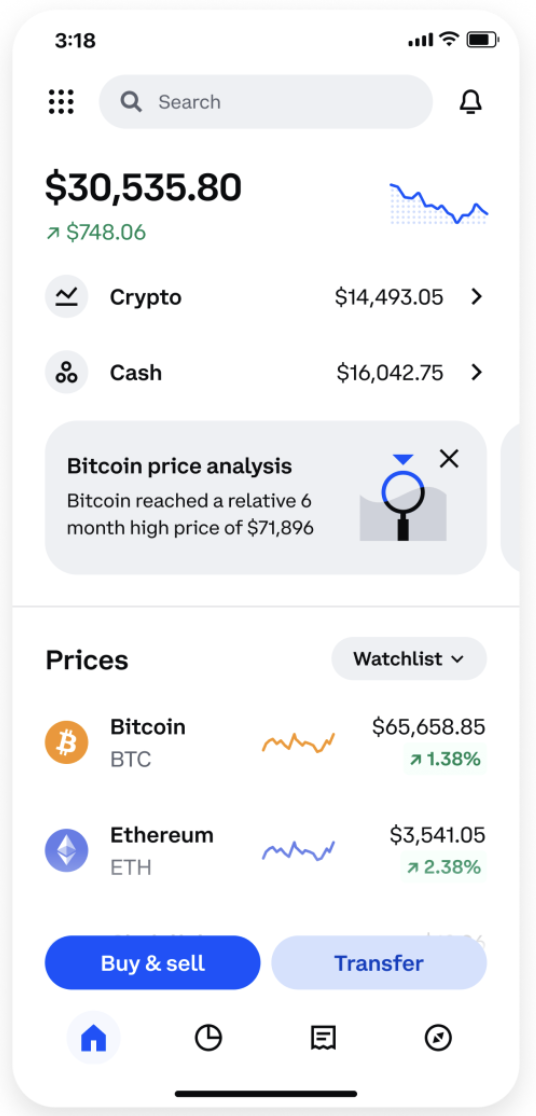
\includegraphics[width=0.4\textwidth]{img/screenshot1.png}
    \caption{Main Dashboard of Coinbase App}
\end{figure}

\subsection{Typography and Readability}
Coinbase uses large, bold fonts to highlight important data such as account balances and cryptocurrency prices, which helps users quickly identify the most relevant information. This practice is particularly effective in mobile contexts where screen space is limited.

\subsection{Iconography and Visual Elements}
The use of intuitive icons and visual elements within the Coinbase app simplifies user interactions by allowing for quick navigation. However, the app could improve by providing additional contextual information or tooltips for less obvious icons.

\begin{figure}[H]
    \centering
    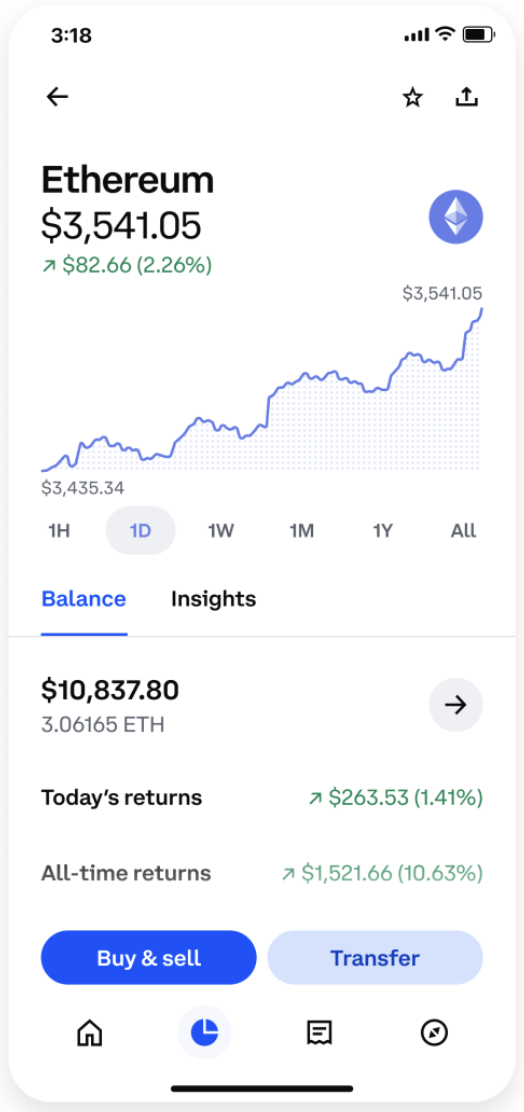
\includegraphics[width=0.4\textwidth]{img/screenshot2.png}
    \caption{Detailed view of Ethereum trading on Coinbase}
\end{figure}

\section{User Experience (UX) Design}

\subsection{Ease of Navigation}
Navigation within the Coinbase app is streamlined through the use of a fixed bottom menu, which is easily accessible with one hand on mobile devices. This is an essential feature in mobile application design, particularly for apps requiring frequent user interaction.

\subsection{Interactivity and Responsiveness}
The Coinbase app excels in interactivity, with responsive buttons and interactive charts that provide immediate feedback to user inputs. These features make the trading experience feel fluid and responsive.

\subsection{Information Accessibility}
Critical information is accessible directly from the main screen, reducing the need to navigate through multiple menus. However, some users may find the initial amount of information overwhelming, suggesting a need for customizable information displays.

\subsection{Adaptation to User Needs}
The ability to customize features such as `Favorites' significantly enhances user engagement by tailoring the app to individual needs. Moreover, real-time notifications and updates are crucial for trading environments but could be optimized to reduce intrusiveness or redundancy.

\section{Notes for our App}
The clear and compartmentalized layout used by Coinbase is ideal for presenting diverse agricultural data in an organized manner. This approach can help users quickly navigate through different categories such as crop yields, market prices, or regional data. Secondly, employing large, bold typography for crucial figures, such as crop prices or weather alerts, will ensure that important information catches the user’s eye immediately, enhancing readability and quick access to vital data. Additionally, the intuitive iconography seen in the Coinbase app can be utilized to help users navigate the app intuitively, with symbols representing different agricultural sectors or operations. Lastly, interactive elements such as dynamic charts and real-time updates could provide users with valuable insights into trends and changes in agricultural metrics, mirroring the interactive financial charts in Coinbase that offer users actionable insights into market trends. Incorporating these elements can make the agricultural metrics app not only informative but also engaging and easy to use, catering effectively to stakeholders involved in Pakistan's agriculture sector.

\end{document}
